\documentclass[12pt]{scrartcl}
\title{Assignment 5\\ Video Report\\ Paper Prototyping}
\author{\textbf{Flow Overstack Team}\\ Cesana Filippo\\ Folli Gary\\ Hartmann Kathrin\\ Rodolfo Masera Tommaso\\ Stucchi Jacopo\\ Taillefert Stefano}
\date{}
\setlength{\parindent}{0pt}

\usepackage{graphicx}
\usepackage{float}
\usepackage[margin = 3cm]{geometry}


\begin{document}

\maketitle

\tableofcontents

\newpage

\section{Introduction}

	% Describe briefly the app idea and refer to our concept statement
	
	TODO (Filippo)

\section{Video Feedback Analysis}
	
	% Analyse and report on data gathered with the one minute video exercise and their implications
	% on our design
	
	\subsection{Expectations versus Reality}
	
		% Summarise what we expected from the children and describe the results we actually got
		% through examples/quotes/etc.
		
		TODO (Stefano)
	
	\subsection{Statistics Analysis}
	
		% Spreadsheet of feedback should go in this subsection
		
		INSERT FIRST PAGE HERE (Tommaso)
		
		\subsubsection*{General tendencies - what’s come out of this globally?}

			Before trying to put our data in a numerical form, we can already look at it to get a general tendency. When we speak about general tendency here, we are not talking about the variance, but simply referring to main ideas or opinions that come out of the data. We were able to identify three general tendencies:

				\paragraph{Application useless and potentially boring in the middle/long term} 
					That was, unfortunately, one of the main tendencies. A certain part of the opinions has pointed out that our application would be simply useless or boring relatively quickly. The problem was that in all these opinions, almost no real reason was given. One was pointing out that he prefers playing “real games” than educative apps and another more interesting opinion admitted that even though he found the idea was great, he would be bored quite quickly due to the fact that the picture taking process is repetitive.

				\paragraph{Application very interesting and original for the learning process and the discovery of history through it}
					Fortunately, there was another main tendency, even more present than the first one, that finds the application really interesting and the idea original. The kids pointed out that the learning process embedded in the app under the form of an interactive game would not only be interesting in term of knowledge but also nice for comparing the portrait with other people. Globally, the children seem quite interested by the famous people especially for the history behind them; some opinions stated that it would be a funny way to learn history. Two children said that they found the idea great because they would discover new areas of interest. This process of learning and discovery was one of the main objectives of the app and thus, hopefully, the children seem to agree on that. 

				\paragraph{Partial or total misunderstanding of the application concept}
					A third tendency, less present than the other two is a partial or total misunderstanding of the app. In other terms, the children did not understand the idea behind the app. Some of them were honest and wrote it, while others, through their comments, were taking the app for something else (a scanner, a snapchat filter extension with old portraits, …). And in our opinion, this tendency is even more present that we think for the simple reason that a lot of opinions were binaries, that is to say, “yes” or “no”; thus probably, a part of these children did not understand well the concepts and simply gave “no” as an answer. After having discussed between us, it is true that our video was probably kind of unclear for the children that were not in the front of the class and instead of putting a music with texts, a voice would have probably helped them understanding the app better.
					
					
		\subsubsection*{Quantitative analysis - can we make the data more readable?}

			By definition, qualitative answers (our data) are more complex to analyze for the simple fact that they are not numbers (scale, ratio, …) and consequently, constructing graphs and other entity making the data more readable becomes harder. Thus, we had to find a way to convert our data in a quantitative way. We decided to get two main ideas out of the data:\\
			
			Do the child like the app? Would they use it?\\

			Both of these opinions are scaled from 0 to 2, 0 being absolutely not, 1 being maybe, 2 being for sure. For every opinion out of the 128, we took the freedom to grade it accordingly to this scale. For us only, we added two more column, a binary one for the writing (if the child writes correctly or not) and one for the class the child was in (first or second class). We wanted the highlight a potential correlation between their ages or their level at school and their opinions on the app. However, we did get any really meaningful correlations. 

			\begin{figure}[H]
                        		\centering
               			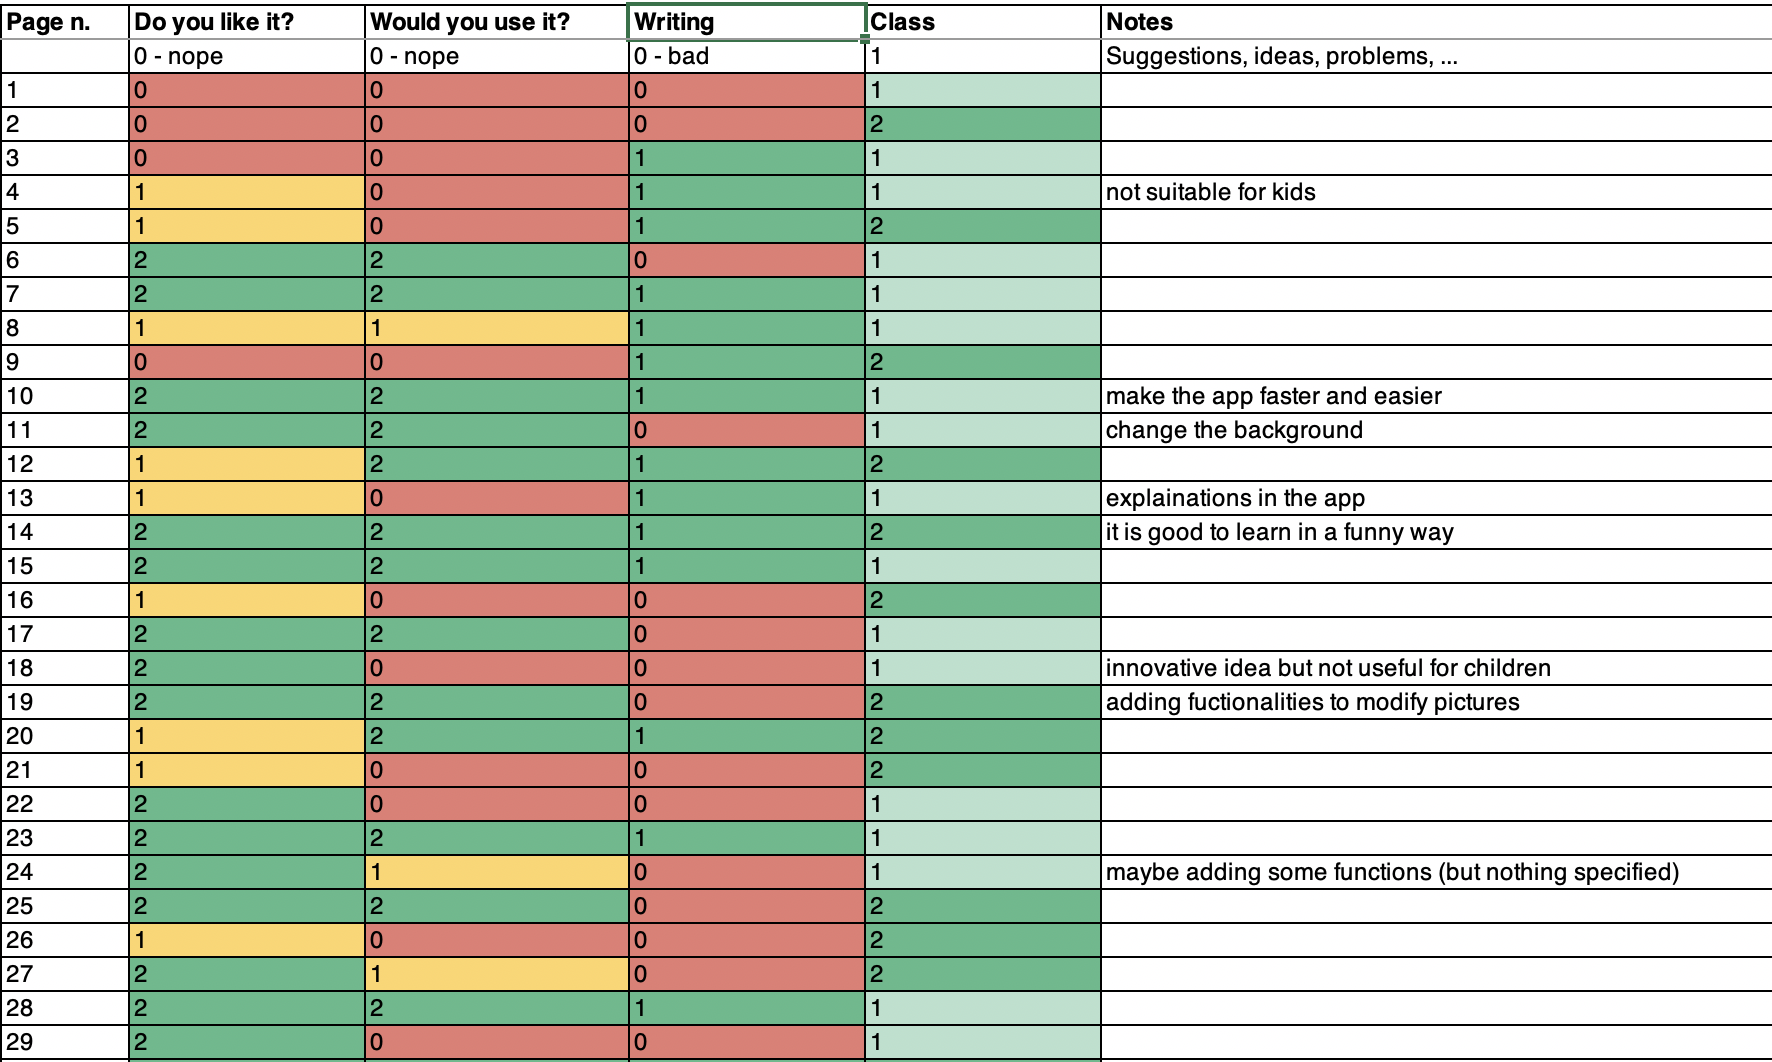
\includegraphics[width=\textwidth]{../images/image_1_data_analysis.png}
               			\caption{TODO}
                        		\label{analysis1}
      			\end{figure}

			Now that we have quantitative data, we can build two graphs in order to make a more robust and precise analysis of our data based on the two questions above. As the scale has a largeness of 3, we choose to represent the data as histograms. To the first question, “do the children like the app?” we got the following histogram. 

			\begin{figure}[H]
                        		\centering
               			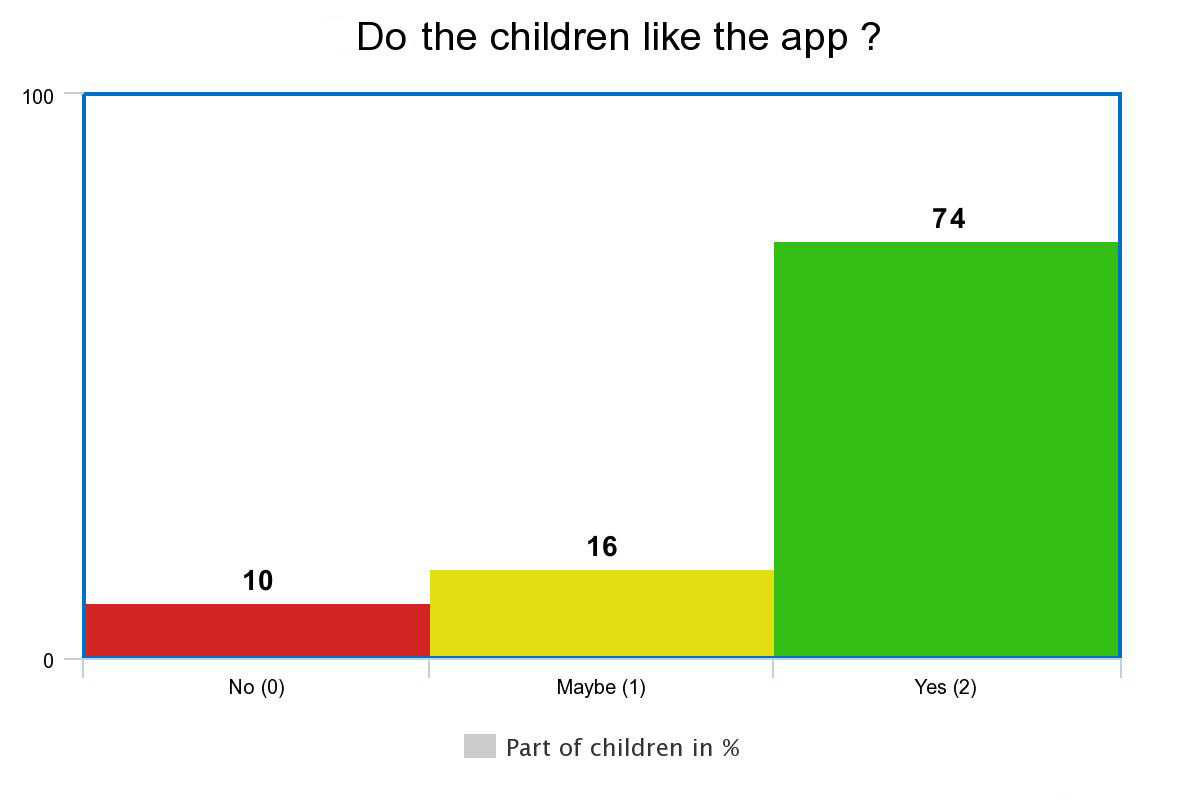
\includegraphics[width=\textwidth]{../images/image_2_data_analysis.jpeg}
               			\caption{TODO}
                        		\label{analysis2}
      			\end{figure}

			This graph shows a net tendency of children liking the app which really show that the idea is considered as interesting and original. Ignoring those that are undecided, we got a rather good percentage of 74 against 10, which means that the majority like the app and find it interesting. Now a better question is, “would the children use it?” and here apparently, we get a sharp difference which shows that the children can like an application without having in mind to use it.\\

			\begin{figure}[H]
                        		\centering
               			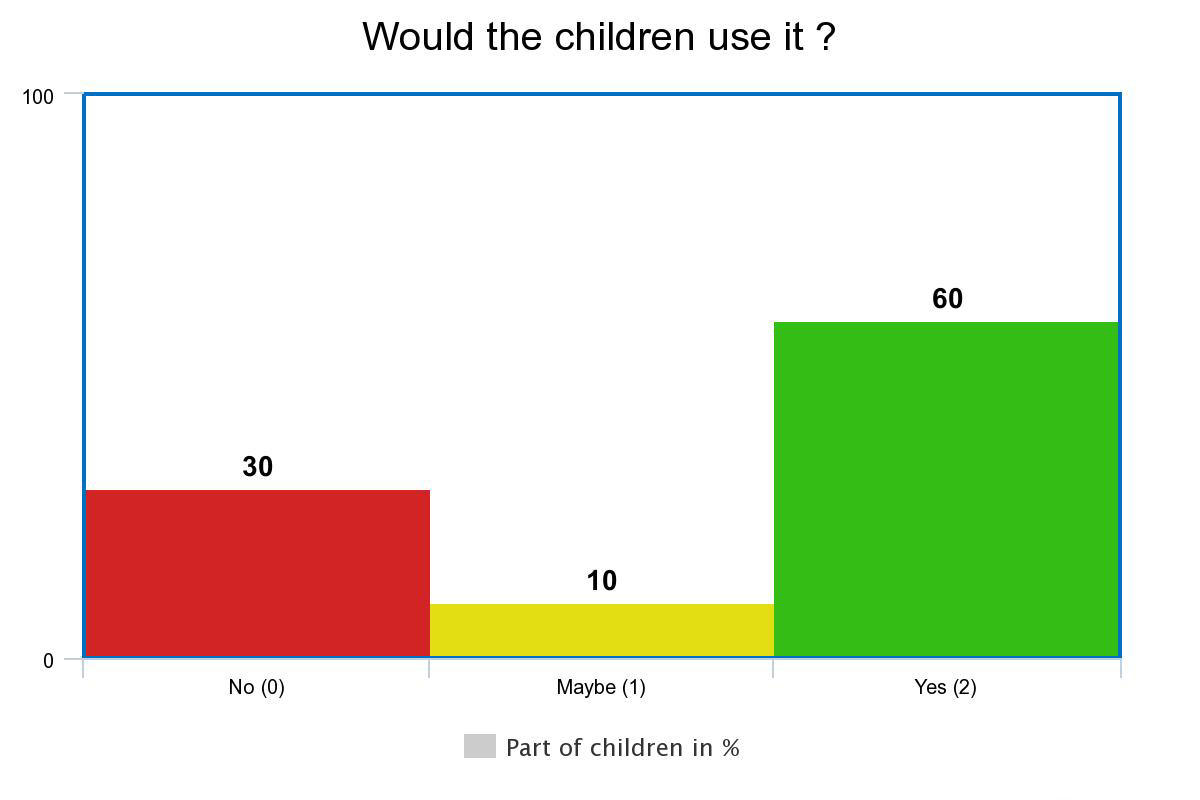
\includegraphics[width=\textwidth]{../images/image_3_data_analysis.jpeg}
               			\caption{TODO}
                        		\label{analysis3}
      			\end{figure}

			Here definitely the tendency is less good, with a small majority of children that would use it against 1/3 of children that would definitely not use it. For the first question, the ratio liked/non-liked was 7, here the ratio is only 2. Thus, even though the children seem to like the app, they are less excited by the idea to use it. As explained in some opinion, the “educative” side seems to be a barrier, indeed, children were explaining studying enough in school and preferring playing for real on their phone and relaxing than continuing learning while playing. We can then clearly see that our app is not unanimous and that even though we try to create a game behind it, the majority of children did not consider it as such.

		
	\subsection{Suggestion-based Improvement}
	
		% Review the kids' feedback and how we plan to modify the project according to it

		Now come the interesting part in having made the questionnaire in such a way that children were able to develop their answers. Although, the majority did not make any comment on it, we got from some children some really good suggestions and potential improvements on the app. Here are those that were the most noteworthy.\\

		One child was pointing out the fact that characteristics of the person could be added in order to improve the matching process. Although it would somehow break the game aspect, it is true that a variant of our app could have been done to be an educative purpose only application used per classroom in which children were asked to choose proposed characteristics (only positive attributes) of their classmates in order for all children in the class to get associated to a given portraits based on their classmate attributes. The teacher would supervise the process and discuss the results with the children and by doing that children would get in contact with famous personages and history though an educative, in-class game.\\
		
		Another child stated that modern VIP should be added in the app as they are more interesting than the past ones. It’s a good idea as modern famous personage would probably add other dimension than history in the app, like science, biology, physics (with Higgs for example). One of its classmates was also pointing out the possibility to add fictional VIP (from films and series) but that would break the educative aspect of the application (adding Jon Snow from Game of Thrones would be not really useful in term of knowledge and history).\\
		
		Another very good opinion stated out that the presence of a search bar would be nice in order to specifically search for a given personage a bit like a Wikipedia of famous personage. That would be an interesting and optional feature for children not interested in the game aspect but more interested by the information and the personages themselves.

	
\section{Paper Prototyping}

	\subsection{Prototype Description}

		% Describe in details the prototype you are creating and how you are going to operate it with 
		% users (peers and children).
		
		TODO (Kathrin \& Tommaso)
		
	\subsection{Key Tasks}
	
		% Show here the list of key tasks (for peers and children) you will use to drive the inspection 
		% process you will run alter on and report in GA6.
	
		TODO (Kathrin \& Tommaso)
			
\section{Conclusion}

	% Describe our expectations for the paper prototype evaluation by the kids/peers
	
	TODO (?)

\end{document}